\documentclass{article}
\usepackage[utf8]{inputenc}
\usepackage{amsmath}
\usepackage{forest}
\usepackage{tikz-qtree}
\usepackage{amssymb}
\usepackage{dirtytalk}
\usepackage{mathtools}
\usepackage{tabularx}
\usepackage{tikz}
\usepackage{xcolor}% or package color
\usetikzlibrary{matrix}
\tikzset{ 
table/.style={
  matrix of nodes,
  row sep=-\pgflinewidth,
  column sep=-\pgflinewidth,
  nodes={rectangle,text width=5em,align=center},
  text depth=1.25ex,
  text height=2.5ex,
  nodes in empty cells
},
row 1/.style={nodes={fill=green!10,text depth=0.4ex,text height=2ex}},
column 1/.style={nodes={fill=green!10}},
}


\usepackage[margin=1.25in]{geometry}

\title{B-splines}
\author{David L. Christensen}
\date{September 2021}

\begin{document}

\maketitle

\section{Introduction}
This paper gives an overview of B splines and how to evaluate them and their derivatives.

\subsection{Nomenclature}


\begin{itemize}
  \item[] d = space dimension of the B-spline curve
  \item[] \textbf{k} = order or degree of the polynomial.
  \item[] n \(=\) number of control points.
  \item[] \textbf{P} = set of control points
  \item[] \(P_i = i^{th}\) control point.
  \item[] m = number of knot points.
  \item[] \textbf{T} = set of knot points 
  \item[] \(t_i = i^{th}\) knot point.
  \item[] \(N_{i , k}\) = basis function for the \(i^{th}\) control point of a \textbf{k} degree B-spline.
  \item[] \(\alpha\) = spacing between uniform knot points
\end{itemize}

\section{Defining B-Splines}

\subsection{Open Uniform B-splines}

\subsubsection{Definition}

 A B-spline or \say{basis spline} is a piece-wise polynomial function of degree \textbf{k}. The formal definition for a b-spline is given by the following equation.
 
  \begin{equation} \label{eq:B-Spline equation}
      b(t) = \sum^{n-1}_{i=0} N_{i,\textbf{k}}(t) P_i
  \end{equation}
 
In words, equation (\ref{eq:B-Spline equation}) defines a b-spline by the summation of the product of some control points \(P_i\) and basis functions \(N_{i,\textbf{k}}(t)\). The basis functions are defined such that each basis function is non-zero only during certain intervals of the b-spline. If we were to evaluate b(t) analytically, we would get a piece-wise polynomial broken up into n-k sections.

\begin{figure}[h]
\begin{center}
\includegraphics[scale=.55]{BsplineVsTime.png}
\end{center}
\caption{B-spline broken up into 5 sections or polynomials. \(t_k = 0\) and \(t_{n} = 5\)}
\label{Fig:B-splines vs time}
\end{figure}

 \begin{equation}
     b(t) = \begin{dcases} 
                p_{\textbf{k}}(t) \quad \textbf{if} \quad t_{\textbf{k}} \leq t < t_{\textbf{k}+1} \\ 
                p_{\textbf{k}+1}(t) \quad \textbf{if} \quad t_{\textbf{k}+1} \leq t < t_{\textbf{k}+2} \\
                \quad ... \\
                p_{n-\textbf{k}}(t)  \quad \textbf{if} \quad t_{n-1} \leq t < t_{n}
            \end{dcases} 
 \end{equation}

Each \(p_j(t)\) is a \(k^{th}\) order polynomial of the form

\begin{equation}
    p_j(t) = c_{j,0} + c_{j,1} \; t + c_{j,2} \; t^{2} + ... + c_{j,k} \; t^{\textbf{k}}
\end{equation}

Also note that the index for the first polynomial starts with \textbf{k} to align the indexing with that of the first defined knot point. This is explained in section \ref{Control and Knot Points}.

\subsubsection{Basis Functions} \label{sec:Basis Functions}

 \begin{figure}[h]
\begin{tabular}{ll}
\includegraphics[scale=.422]{BasisFunctionsOrder2.png}
\\
\includegraphics[scale=.42]{BasisFunctionsOrder5.png}
\end{tabular}
\caption{$2^{nd}$ and $5^{th}$ order Basis functions with ten control points}
\label{Fig:Open Basis Functions}
\end{figure}

  The basis function \(N_{i,\kappa(t)}\) is defined using the Cox-de Boor recursion formula as shown below.
  
  \begin{equation} \label{eq:Basis function equation}
  N_{i,\kappa}(t) = \frac{t - t_i}{t_{i+\kappa} - t_i} N_{i,\kappa-1}(t) + \frac{t_{i+\kappa+1} - t}{t_{i+\kappa+1}-t_{i+1}} N_{i+1 , \kappa-1}(t)    
  \end{equation}
  
    \begin{equation} \label{eq:Basis function equation zeros}
      N_{i,0} =   \begin{cases} 1, &  \text{if } t_i \leq t < t_{i+1} \\
                            0, & \text{otherwise} \end{cases}
  \end{equation}
  
  If we were to evaluate a basis function analytically, we would get a polynomial of the following form.
  
  \begin{equation}
      N_{i,\textbf{k}}(t) = c_{i,0} + c_{i,1} \; t + c_{i,2} \; t^{2} + ... + c_{i,3} \; t^{\textbf{k}}
  \end{equation}
  
  A B-spline has a total of n basis functions. Each basis function influences k+1 intervals of the piece-wise polynomial. We can see this from Figure (\ref{Fig:Open Basis Functions}), which shows plots of the basis functions for a second and fifth order b-spline. These b-splines each have ten control points and each polynomial piece is defined over a one second interval. In the second order graph, each interval has three active basis functions, and in the fifth order graph, each interval has six active basis functions. In other words, each polynomial piece \(p(t)\) is defined by \textbf{k}+1 basis functions. 
  
\begin{equation}
    p_j(t) = N_{j,\textbf{k}} P_{j} \; + \; N_{j-1,\textbf{k}} P_{j-1} \; + \; ... \; + \; N_{j-\textbf{k},\textbf{k}} P_{j-\textbf{k}}
\end{equation}

\subsubsection{Control and Knot Points} \label{Control and Knot Points}

\begin{figure}[h]
\begin{tabular}{ll}
\includegraphics[scale=.4]{2ndOrderBspline.png}
&
\includegraphics[scale=.4]{5th Order B-spline.png}
\end{tabular}
\caption{$2^{nd}$ and $5^{th}$ order B-splines in 2 dimensions}
\label{Fig:Uniform B-splines}
\end{figure}

The reason that we define a piece-wise polynomial in the B-spline form is so that we can take advantage of knot and control points. Knot points are required to define the time intervals for which each polynomial piece is defined. Knot points of a uniform B-spline must adhere to the following rules.

\begin{equation}
    \begin{aligned}
        & t_i < t_{i+1} \\
        & t_{i+1} - t_i = t_{i} - t_{i-1}
    \end{aligned}
\end{equation}

\begin{equation}
    t_i \in \mathbb{R} 
\end{equation}

where the uniform spacing between knot points is given by \(\alpha\).

\begin{equation}
    \alpha = t_{i+1} - t_i
\end{equation}


Given a set \textbf{P} of (n) control points

\begin{equation}
    \textbf{P} = \begin{bmatrix} P_0, & P_1, & ... & P_{n-1} \end{bmatrix}
\end{equation}

We must have a set \textbf{T} of (m) equally spaced knot points.

\begin{equation}
    \textbf{T} = \begin{bmatrix} t_0, & t_1 , & ... & t_{m-1} \end{bmatrix}
\end{equation}

where 

\begin{equation}
    m = n + k + 1
\end{equation}

Figure (\ref{Fig:Uniform B-splines}) shows a \(2^{nd}\) and \(5^{th}\) order uniform B-spline. We note that the B-spline is defined only between the knot points \(t_k\) and \(t_n\), where each interval \([t_i , t_{i+1})\) describes one of the polynomials that make up the B-spline. This gives us n-\textbf{k} knot point intervals in the curve.

\begin{equation}
    \Big[ t_0, \; t_1,  \; ... \; t_{k-1} , \; \underbrace{t_k, \; t_{k+1}, \; ... \; t_n,}_{\text{defined}} \; t_{m-k}, \; t_{m-k+1}, \; ... \; t_{m-1} \Big]
\end{equation}

Control points shape the physical coordinates of the spline (see Figure \ref{Fig:Uniform B-splines}). The dimension or coordinate space that the control points reside in determine the dimension of the B-spline. For a d dimensional control point we have
 
 \begin{equation}
     P_i \in \mathbb{R}^{d \times 1}
 \end{equation}
 
For a 3 dimensional spline we would have
 
  \begin{equation}
     P_i = \begin{bmatrix} P_{x_i} \\ P_{y_i} \\ P_{z_i} \end{bmatrix}
 \end{equation}
 
In section \ref{sec:Basis Functions}, we note that the number of control points is equal to the number of basis functions, and therefore each spline section \(p_j(t)\) is defined by \textbf{k}+1 control points. Specifically, the polynomial in the interval \([t_{i+\textbf{k}} , t_{i+\textbf{k}+1}]\) is effected by control points \([P_i , P_{i+1}, ... P_{i+\textbf{k}}]\). This means at least \textbf{k}+1 control points are needed to define a B-spline.

\subsection{Clamped Uniform B-splines}

\begin{figure}[h]
\begin{tabular}{ll}
\includegraphics[scale=.4]{2ndOrderClampedBspline.png}
&
\includegraphics[scale=.4]{5thOrderClampedBspline.png}
\end{tabular}
\caption{$2^{nd}$ and $5^{th}$ order clamped B-splines in 2 dimensions}
\label{Fig:Race}
\end{figure}

A clamped B-spline, or open uniform B-spline is a one that reaches its first and last control points. We can create a clamped B-spline by enforcing the following constraints to the knot points.

\begin{equation}
\begin{aligned}
    t_\textbf{k} & = \quad t_0 = t_1 = ... \; t_{\textbf{k}-1} \\
    t_n & = \quad  t_{m-k} = t_{m-k+1} = ... \; t_{m-1}
\end{aligned}
\end{equation}

\begin{equation}
    t_i \leq t_{i+1}
\end{equation}

The B-spline equations remains the same.

  \begin{equation}
      b(t) = \sum^{n-1}_{i=0} N_{i,\textbf{k}}(t) P_i
  \end{equation}

However the basis function changes slightly to avoid division by zero.


  \begin{equation} \label{eq:Basis function equation}
  N_{i,\kappa}(t) = \begin{dcases}  \quad 0 \quad  \textbf{if } \quad t_{i+1} = t_{i+k+1} \quad  \textbf{ and } \quad t_{i+k} = t_{i} \\  \\ \frac{t - t_i}{t_{i+\kappa} - t_i} N_{i,\kappa-1}(t) \quad  \textbf{else if } \quad t_{i+1} = t_{i+k+1} \\ \\ 
  \frac{t_{i+\kappa+1} - t}{t_{i+\kappa+1}-t_{i+1}} N_{i+1 , \kappa-1}(t) \quad \textbf{else if} \quad t_{i+k} = t_{i} \\ \\
  \frac{t - t_i}{t_{i+\kappa} - t_i} N_{i,\kappa-1}(t) + \frac{t_{i+\kappa+1} - t}{t_{i+\kappa+1}-t_{i+1}} N_{i+1 , \kappa-1}(t) \quad \textbf{otherwise}
  \end{dcases}
  \end{equation}
  
 \hspace{1cm}
 
 \begin{equation} \label{eq:Basis function equation zeros}
      N_{i,0} =   \begin{cases} 1, &  \text{if } \quad t_i \leq t < t_{i+1} \\
                            1, & \text{if } \quad t_i \leq t = t_{i+1} = t_n \\
                            0, & \text{otherwise} \end{cases}
  \end{equation}
  
\section{Evaluating B-Splines}

\subsection{Recursive Evaluation}

To evaluate a B-spline at a time \(t_p\), where

\begin{equation}
  t_{j} \leq t_p \le t_{j+1}
\end{equation}

equation (\ref{eq:B-Spline equation}) only needs to be computed for knot points \([P_{j-\textbf{k}}, P_{j-\textbf{k}+1}, ... P_j]\)

\begin{equation}
    b(t_p) = \sum^{j}_{i=j-k} N_{i,\textbf{k}} P_i
\end{equation}

where a graphical representation of \(N_{i,\textbf{k}}\) is shown below.
 
\hspace{1cm}

\begin{forest}
    [\(N_{i,\kappa}\)
          [\(f_{i,\kappa}N_{i,\kappa-1}\)
             [\(f_{i,\kappa-1}N_{i,\kappa-2}\)[...[\(f_{i,1}N_{i,0}\)][...]][...[...][...]]]
             [\(d_{i,\kappa-1}N_{i+1,\kappa-2}\)[...[...][...]][...[...][...]]]]
          [\(d_{i,\kappa}N_{i+1,\kappa-1}\)
             [\(f_{i+1,\kappa-1}N_{i+1,\kappa-2}\)[...[...][...]][...[...][...]]]
             [\(d_{i+1,\kappa-1}N_{i+2,\kappa-2}\)[...[...][...]][...[...][\(d_{i+k-1,1} N_{i+\kappa,0}\)]]]
    ]]
\end{forest}

\hspace{1cm}

where

\begin{equation}
    f_{i,\kappa} = \frac{t - t_i}{t_{i+\kappa}- t_i} \quad , \quad d_{i,\kappa} = \frac{t_{i+\kappa+1} - t}{t_{i+\kappa+1}-t_{i+1}}
\end{equation}

\hspace{1cm}

Table ( ) shows the psuedocode for this implementation.

TODO

\subsection{Triangular Scheme Method}

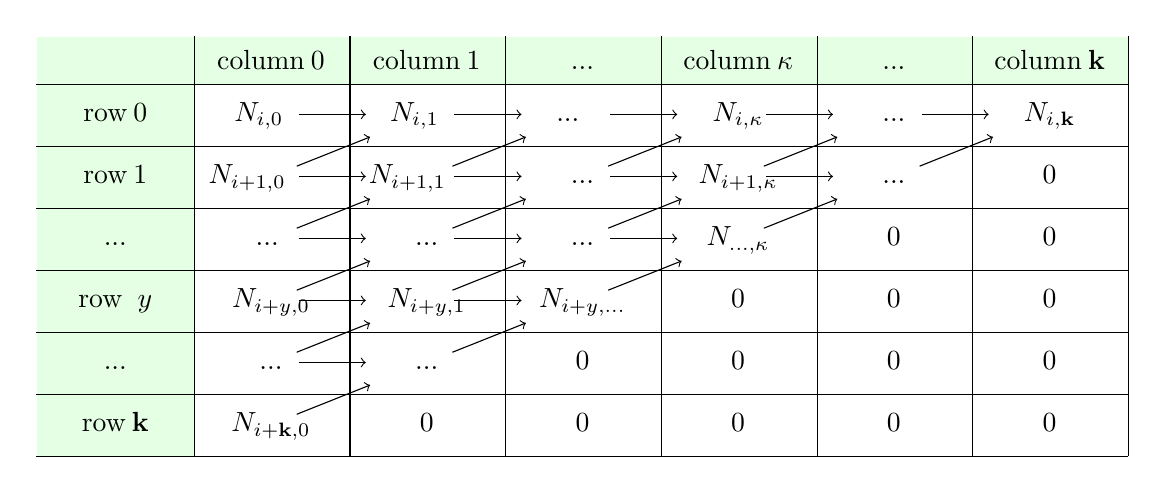
\begin{tikzpicture}
% the matrix entries
\matrix (mat) [table]
{
& column\:0 & column\:1 & ... & column\:$\kappa$ & ... & column\:\textbf{k} \\
row\:0 & $N_{i,0} \;\; $  & $N_{i,1} \;\; $ & ... \;\;  & $ N_{i,\kappa}$ & ... & $ N_{i,\textbf{k}}$\\
row\:1 & $N_{i+1,0}$ \;\;\;\;\; & $N_{i+1,1}$\;\;\;\;\; & ... & $ N_{i+1,\kappa}$ & ... & 0\\
... & ...\; & ... & ... & $N_{...,\kappa}$ & 0 & 0\\
row\: $y$ & $N_{i+y,0}$ & $N_{i+y,1}$ & $N_{i+y,...}$ & 0 & 0 & 0\\
... & ... & ... & 0 & 0 & 0 & 0\\
row\:\textbf{k} & $N_{i+\textbf{k},0}$ & 0 & 0 & 0 & 0 & 0\\
};
% the matrix rules
\foreach \x in {1,...,7}
{
  \draw 
    ([xshift=-.5\pgflinewidth]mat-\x-1.south west) --   
    ([xshift=-.5\pgflinewidth]mat-\x-7.south east);
  }
\foreach \x in {1,...,7}
{
  \draw 
    ([yshift=.5\pgflinewidth]mat-1-\x.north east) -- 
    ([yshift=.5\pgflinewidth]mat-7-\x.south east);
}    
% the arrows
\begin{scope}[shorten >=22pt,shorten <= 10pt]
\draw[->]  (mat-2-2.center) -- (mat-2-3.center);
\draw[->]  (mat-2-3.center) -- (mat-2-4.center);
\draw[->]  (mat-2-4.center) -- (mat-2-5.center);
\draw[->]  (mat-2-5.center) -- (mat-2-6.center);
\draw[->]  (mat-2-6.center) -- (mat-2-7.center);
\draw[->]  (mat-3-2.center) -- (mat-3-3.center);
\draw[->]  (mat-3-3.center) -- (mat-3-4.center);
\draw[->]  (mat-3-4.center) -- (mat-3-5.center);
\draw[->]  (mat-3-5.center) -- (mat-3-6.center);
\draw[->]  (mat-4-2.center) -- (mat-4-3.center);
\draw[->]  (mat-4-3.center) -- (mat-4-4.center);
\draw[->]  (mat-4-4.center) -- (mat-4-5.center);
\draw[->]  (mat-5-2.center) -- (mat-5-3.center);
\draw[->]  (mat-5-3.center) -- (mat-5-4.center);
\draw[->]  (mat-6-2.center) -- (mat-6-3.center);

\draw[->]  (mat-7-2.center) -- (mat-6-3.center);
\draw[->]  (mat-6-2.center) -- (mat-5-3.center);
\draw[->]  (mat-6-3.center) -- (mat-5-4.center);
\draw[->]  (mat-5-2.center) -- (mat-4-3.center);
\draw[->]  (mat-5-3.center) -- (mat-4-4.center);
\draw[->]  (mat-5-4.center) -- (mat-4-5.center);
\draw[->]  (mat-4-2.center) -- (mat-3-3.center);
\draw[->]  (mat-4-3.center) -- (mat-3-4.center);
\draw[->]  (mat-4-4.center) -- (mat-3-5.center);
\draw[->]  (mat-4-5.center) -- (mat-3-6.center);
\draw[->]  (mat-3-2.center) -- (mat-2-3.center);
\draw[->]  (mat-3-3.center) -- (mat-2-4.center);
\draw[->]  (mat-3-4.center) -- (mat-2-5.center);
\draw[->]  (mat-3-5.center) -- (mat-2-6.center);
\draw[->]  (mat-3-6.center) -- (mat-2-7.center);


\end{scope}
\end{tikzpicture}

\begin{equation}
    \rightarrow \:\: = \: \times \; \frac{t - t_{i+y}}{t_{i+y+\kappa} - t_{i+y}} \; + 
\end{equation}

\begin{equation}
    \nearrow \:\:  = \times \; \frac{t_{i+y+\kappa+1} - t}{t_{i+y+\kappa+1}-t_{i+y+1}} \; + 
\end{equation}

If we call the table \say{N}, then we have each cell of the table equal to the following.

\begin{equation}
    N[y,\kappa] = \frac{t - t_{i+y}}{t_{i+y+\kappa} - t_{i+y}} N[y,\kappa-1] + \frac{t_{i+y+\kappa+1} - t}{t_{i+y+\kappa+1}-t_{i+y+1}} N[y+1,\kappa-1]
\end{equation}

\begin{equation} \label{eq:Basis function equation zeros}
      N[y,0] =   \begin{cases} 1, &  \text{if} \quad t_{i+y} \leq t < t_{i+y+1} \\
                            0, & \text{otherwise} \end{cases}
  \end{equation}
  
 Table () shows the psuedocode for this implementation.
 
 TODO

\subsection{Matrix Method}
    \subsubsection{General Equations}
    
OPEN UNIFORM B-SP\GammaINES
\hfill \break
    
    \begin{equation}
        b(t) = \textbf{B} M L
    \end{equation}

        where
    
    \begin{equation}
    M \in \mathbb{R}^{\textbf{k}+1 \times \textbf{k}+1}
    \end{equation}
        
    \begin{equation}
        \textbf{B} = \begin{bmatrix} P_{i} & P_{i+1} & ... & P_{i+\textbf{k}}\end{bmatrix}
    \end{equation}
    
    \begin{equation}
        L = \begin{bmatrix} \tau^{\textbf{k}} \\ ... \\ \\ \tau^2 \\ \tau \\ 1 \end{bmatrix}
    \end{equation}
    
    where
    
    \begin{equation}
        \tau = \frac{t-t_j}{\alpha}
    \end{equation}
    
    and
    
    \begin{equation}
        t_j \leq t < t_{j+1} \quad , \quad i = j-\textbf{k}
    \end{equation}
    
Also note that \(M\) is a matrix of constants, unique for the order of the B-spline. An expanded form of the equation is shown below.

\begin{equation}
    c_0 + c_1 t + c_2 t^2 + ... + c_{\textbf{k}} t^{\textbf{k}} = \begin{bmatrix} P_{i} & P_{i+1} & ... & P_{i+\textbf{k}}\end{bmatrix} M \begin{bmatrix} (\frac{t-t_j}{\alpha})^\textbf{k} \\ \\ ... \\ \\ (\frac{t-t_j}{\alpha})^2 \\ \\ (\frac{t-t_j}{\alpha}) \\ \\ 1 \end{bmatrix}
\end{equation}

\noindent CLAMPED UNIFORM B-SPLINES
\hfill \break

For a clamped B-spline, the \(M\) matrix takes on different values when defined over the beginning and ending intervals. For a \(\textbf{k}^{th}\) order B-spline we have will have up to \(2\textbf{k}-1\) different matrices.


\begin{equation} 
        M = \begin{dcases} 
            M_{1} \quad \text{for} \quad t_{\textbf{k}} \leq t < t_{\textbf{k}+1} \\
            M_{2} \quad \text{for} \quad t_{\textbf{k}+1} \leq t < t_{\textbf{k}+2} \\
            ...\\
            M_{\textbf{k}} \quad \text{for} \quad t_{2\textbf{k}-1} \leq t < t_{n-\textbf{k}+1}\\
            ...\\
            M_{2\textbf{k}-2} \quad \text{for} \quad t_{n-2} \leq t < t_{n-1}\\
            M_{2\textbf{k}-1} \quad \text{for} \quad t_{n-1} \leq t < t_{n}
        \end{dcases}
\end{equation}

given

    \begin{equation}
        \textbf{P} = \begin{bmatrix} P_0, P_1, ... P_{n-1} \end{bmatrix} \quad \text{,} \quad n \geq 3\textbf{k}-1
    \end{equation}
    
    \begin{equation}
        \textbf{T} = \begin{bmatrix} t_0, t_1, ... t_{m-1} \end{bmatrix} \quad \text{,} \quad m \geq 4\textbf{k}
    \end{equation}

\begin{equation}
    m = n+\textbf{k}+1
\end{equation}

If we reduce the number of control points below \(3\textbf{k}-1\), we reduce the number of matrices required to make up the b-spline. Figure (\ref{Fig:ClampedMatricesWithReducedN}) shows how many, and what matrices are needed for a certain number of control points. \(\mu\) is the number of matrices required.

\begin{figure}[h]
\begin{tabular}{ll}
\includegraphics[scale=.32]{ClampedMatricesReducedN.png}
\end{tabular}
\caption{A diagram of the matrices required for a specific number of control points}
\label{Fig:ClampedMatricesWithReducedN}
\end{figure}

We can define the \(M\) matrix by including additional checks, and by defining new center matrices \(M_c\). The minimum amount of control points required for a \(\textbf{k}^{th}\) order B-spline is \(\textbf{k}+1\), where we would have just one matrix, and one polynomial to describe the spline.

\begin{equation} 
        M = \begin{dcases} 
            M_{1} \quad \text{for} \quad t_{\textbf{k}} \leq t < t_{\textbf{k}+1} \quad \text{and} \quad t_\textbf{k} < t_{n-1} \\
            M_{2} \quad \text{for} \quad t_{\textbf{k}+1} \leq t < t_{\textbf{k}+2} \quad \text{and} \quad t_{\textbf{k}+1} < t_{n-2} \\
            ...\\
            M_{c} \quad \text{for} \quad \text{n-\textbf{k} is odd} \quad \text{or} \quad n \geq 3\textbf{k}-1 \\
            ...\\
            M_{2\textbf{k}-2} \quad \text{for} \quad t_{n-2} \leq t < t_{n-1} \quad \text{and} \quad t_{\textbf{k}+1} < t_{n-2}\\
            M_{2\textbf{k}-1} \quad \text{for} \quad t_{n-1} \leq t < t_{n} \quad \text{and} \quad t_\textbf{k} < t_{n-1}
        \end{dcases}
\end{equation}

\begin{equation} 
        M_c = \begin{dcases} 
            M_{c_1} \quad \text{for} \quad t_{2\textbf{k}-1} \leq t < t_{n-\textbf{k}+1} \quad \text{and} \quad t_{2\textbf{k}-1} \leq  t_{n-\textbf{k}}\\
            M_{c_2} \quad \text{for} \quad t_{2\textbf{k}-2} \leq t < t_{n-\textbf{k}+2} \quad \text{and} \quad t_{2\textbf{k}-2} = t_{n-\textbf{k}+1}\\
            ...\\
            M_{c_\textbf{k}} \quad \text{for} \quad t_{\textbf{k}} \leq t < t_{n} \quad \text{and} \quad t_\textbf{k} = t_{n-1}
        \end{dcases}
\end{equation}

given

    \begin{equation}
        \textbf{P} = \begin{bmatrix} P_0, P_1, ... P_{n-1} \end{bmatrix} \quad \text{,} \quad n \geq \textbf{k}+1
    \end{equation}
    
    \begin{equation}
        \textbf{T} = \begin{bmatrix} t_0, t_1, ... t_{m-1} \end{bmatrix} \quad \text{,} \quad m \geq 2(\textbf{k} + 1)
    \end{equation}

\subsubsection{Linear Splines}

LINEAR B-SPLINES
\hfill \break

    The matrix equation for a uniform linear B-Spline. This following equation applies to both open and clamped linear B-splines.
    
    \begin{equation}
        b(t) = \begin{bmatrix} P_i & P_{i+1} \end{bmatrix} \begin{bmatrix} -1 & 1 \\ 1 & 0
        \end{bmatrix} \begin{bmatrix} \tau^2 \\ \tau \\ 1 \end{bmatrix}
    \end{equation}
    
    for
    
    \begin{equation}
        \tau = \frac{t-t_j}{\alpha}
    \end{equation}
    
    \begin{equation}
        t_j < t < t_{j+1} \quad , \quad i = j-\textbf{k}
    \end{equation}
    
    where 
    
    \begin{equation}
    M_{\textbf{k}} = \begin{bmatrix} -1 & 1 \\ 1 & 0
        \end{bmatrix}
    \end{equation}
    
    \begin{equation}
        L = \begin{bmatrix} \tau & 1 \end{bmatrix}^{T}
    \end{equation}
    
    \begin{equation}
        \textbf{B} = \begin{bmatrix} P_{i} & P_{i+1}\end{bmatrix}
    \end{equation}
    
    given
    
    \begin{equation}
    \textbf{P} = \begin{bmatrix} P_0, P_1, ... P_{n-1} \end{bmatrix} \quad \text{,} \quad n \geq 2
    \end{equation}
    
    \begin{equation}
        \textbf{T} = \begin{bmatrix} t_0, t_1, ... t_{m-1} \end{bmatrix} \quad \text{,} \quad m \geq 4
    \end{equation}

\subsubsection{Quadratic Splines}
   
OPEN QUADRATIC B-SPLINES
\hfill \break

    The matrix equation for a uniform quadratic B-Spline.
    
    \begin{equation}
        b(t) = \begin{bmatrix} P_i & P_{i+1} & P_{i+2} \end{bmatrix} \frac{1}{2} \begin{bmatrix} 1 & -2 & 1 \\ -2 & 2 & 1 \\ 1 & 0 & 0
        \end{bmatrix} \begin{bmatrix} \tau^2 \\ \tau \\ 1 \end{bmatrix}
    \end{equation}
    
    for
    
    \begin{equation}
        \tau = \frac{t-t_j}{\alpha}
    \end{equation}
    
    \begin{equation}
        t_j < t < t_{j+1} \quad , \quad i = j-\textbf{k}
    \end{equation}
    
    where 
    
    \begin{equation}
    M_{\textbf{k}} = \frac{1}{2}\begin{bmatrix}
                        1 & -2 & 1 \\
                       -2 &  2 & 1 \\
                        1 &  0 & 0
                    \end{bmatrix}
    \end{equation}
    
    \begin{equation}
        L = \begin{bmatrix} \tau^{2} & \tau & 1 \end{bmatrix}^{T}
    \end{equation}
    
    \begin{equation}
        \textbf{B} = \begin{bmatrix} P_{i} & P_{i+1} & P_{i+2}\end{bmatrix}
    \end{equation}
    
    given
    
    \begin{equation}
    \textbf{P} = \begin{bmatrix} P_0, P_1, ... P_{n-1} \end{bmatrix} \quad \text{,} \quad n \geq 3
    \end{equation}
    
    \begin{equation}
        \textbf{T} = \begin{bmatrix} t_0, t_1, ... t_{m-1} \end{bmatrix} \quad \text{,} \quad m \geq 6
    \end{equation}
    
    
\noindent CLAMPED QUADRATIC B-SPLINES
\hfill \break

    Below we define the M matrix over specific intervals of the Clamped B-spline. With 5 or more control points (n), the total number of matrices (\(\mu\)) needed to define the B-spline is 3. The number of matrices (\(\mu\)) decreases as we decrease the number of control points below 5.
    
    \begin{equation}
        M = \begin{dcases} 
            \frac{1}{2}\begin{bmatrix} 2 & -4 & 2 \\
                                        -3 & 4 & 0 \\
                                        1 & 0 & 0 \end{bmatrix} \quad \text{for} \quad t_2 \leq t < t_{3} \quad \text{and} \quad t_2 < t_{n-1}\\\\
            M_c \quad \text{for} \quad \text{n-2 is odd} \quad \text{or} \quad n \geq 5 \\\\
            \frac{1}{2} \begin{bmatrix} 1 & -2 & 1 \\
                                        -3 & 2 & 1 \\
                                        2 & 0 & 0 \end{bmatrix} \quad \text{for} \quad t_{n-1} \leq t < t_{n} \quad \text{and} \quad t_2 < t_{n-1}
        \end{dcases}
    \end{equation}
    
    \begin{equation}
        M_c = \begin{dcases} 
            \frac{1}{2}\begin{bmatrix} 1 & -2 & 1 \\
                                        -2 & 2 & 1 \\
                                        1 & 0 & 0 \end{bmatrix} \quad \text{for} \quad t_{3} \leq t < t_{n-1} \quad \text{and} \quad t_3 \leq t_{n-2}\\\\
            \frac{1}{2} \begin{bmatrix} 2 & -4 & 2 \\
                                        -4 & 4 & 0 \\
                                        2 & 0 & 0 \end{bmatrix} \quad \text{for} \quad t_{2} \leq t < t_{n}  \quad \text{and} \quad t_2 = t_{n-1}
        \end{dcases}
    \end{equation}

        given
    
   \begin{equation}
        \textbf{P} = \begin{bmatrix} P_0, P_1, ... P_{n-1} \end{bmatrix} \quad \text{and} \quad n \geq 3
    \end{equation}
    
    \begin{equation}
        \textbf{T} = \begin{bmatrix} t_0, t_1, ... t_{m-1} \end{bmatrix} \quad \text{and} \quad m \geq 6
    \end{equation}
    
    
    \subsubsection{Cubic Splines}
    
OPEN CUBIC B-SPLINES
\hfill \break

    The matrix equation for a uniform quadratic B-Spline.
    
    \begin{equation}
        b(t) = \begin{bmatrix} P_i & P_{i+1} & P_{i+2} & P_{i+3} \end{bmatrix} \frac{1}{12} \begin{bmatrix} -2 & 6 & -6 & 2 \\
                                          6 & -12 & 0 & 8 \\
                                         -6 & 6 & 6 & 2 \\
                                          2 & 0 & 0 & 0 \end{bmatrix} \begin{bmatrix} \tau^3 \\ \tau^2 \\ \tau \\ 1 \end{bmatrix}
    \end{equation}
    
    for
    
    \begin{equation}
        \tau = \frac{t-t_j}{\alpha}
    \end{equation}
    
    \begin{equation}
        t_j < t < t_{j+1} \quad , \quad i = j-\textbf{k}
    \end{equation}
    
    where 
    
    \begin{equation}
    M = \frac{1}{12} \begin{bmatrix} -2 & 6 & -6 & 2 \\
                                          6 & -12 & 0 & 8 \\
                                         -6 & 6 & 6 & 2 \\
                                          2 & 0 & 0 & 0 \end{bmatrix}
    \end{equation}
    
    \begin{equation}
        L = \begin{bmatrix} \tau^{3} & \tau^{2} & \tau & 1 \end{bmatrix}^{T}
    \end{equation}
    
    \begin{equation}
        \textbf{B} = \begin{bmatrix} P_{i} & P_{i+1} & P_{i+2} & P_{i+3}\end{bmatrix}
    \end{equation}
    
    given
    
    \begin{equation}
    \textbf{P} = \begin{bmatrix} P_0, P_1, ... P_{n-1} \end{bmatrix} \quad \text{,} \quad n \geq 4
    \end{equation}
    
    \begin{equation}
        \textbf{T} = \begin{bmatrix} t_0, t_1, ... t_{m-1} \end{bmatrix} \quad \text{,} \quad m \geq 8
    \end{equation}
    
    
\noindent CLAMPED CUBIC B-SPLINES
\hfill \break

    Below we define the M matrix over specific intervals of the Clamped B-spline. With 8 or more control points (n), the total number of matrices (\(\mu\)) needed to define the B-spline is 5. The number of matrices (\(\mu\)) decreases as we decrease the number of control points below 8.

    \begin{equation}
        M = \begin{dcases} 
            \frac{1}{12}\begin{bmatrix} -12 &  36 & -36 & 12 \\
                                         21 & -54 &  36 & 0 \\
                                        -11 &  18 &  0  & 0 \\
                                         2  &   0 &  0  & 0 \end{bmatrix} \quad \text{for} \quad t_3 \leq t < t_{4} \quad \text{and} \quad t_3 = t_{n-1}\\\\
            \frac{1}{12}\begin{bmatrix} -3 &  9  & -9 & 3 \\
                                         7 & -15 &  3 & 7 \\
                                        -6 &  6  &  6 & 2 \\
                                         2 &  0  &  0 & 0 \end{bmatrix} \quad \text{for} \quad t_{4} \leq t < t_{5} \quad \text{and} \quad t_4 = t_{n-2}\\\\
            M_c \quad \text{for} \quad \text{n-3 is odd} \quad \text{or} \quad n\geq 8 \\\\
            \frac{1}{12} \begin{bmatrix} -2 & 6 & -6 & 2 \\
                                          6 & -12 & 0 & 8 \\
                                         -7 & 6 & 6 & 2 \\
                                          3 & 0 & 0 & 0
                                      \end{bmatrix} \quad \text{for} \quad t_{n-2} \leq t < t_{n-1} \quad \text{and} \quad t_4 = t_{n-2} \\\\
            \frac{1}{12} \begin{bmatrix} -2 & 6 & -6 & 2 \\
                                         11 & -15 & -3 & 7 \\
                                        -21 & 9 & 9 & 3 \\
                                         12 & 0 & 0 & 0
                                      \end{bmatrix} \quad \text{for} \quad t_{n-1} \leq t < t_{n} \quad \text{and} \quad t_3 = t_{n-1}
            \end{dcases}
    \end{equation}
    
    \begin{equation}
        M_c = \begin{dcases} 
            \frac{1}{12} \begin{bmatrix} -2 & 6 & -6 & 2 \\
                                          6 & -12 & 0 & 8 \\
                                         -6 & 6 & 6 & 2 \\
                                          2 & 0 & 0 & 0 \end{bmatrix} \quad \text{for} \quad t_{5} \leq t < t_{n-2} \quad \text{and} \quad t_5 \leq t_{n-3}\\\\
            \frac{1}{12} \begin{bmatrix} -3 & 9 & -9 & 3 \\
                                          7 & -15 & 3 & 7 \\
                                         -7 & 6 & 6 & 2 \\
                                          3 & 0 & 0 & 0 \end{bmatrix} \quad \text{for} \quad t_{4} \leq t < t_{n-1} \quad \text{and} \quad t_4 = t_{n-2}\\\\
            \frac{1}{12} \begin{bmatrix} -12 & 36 & -36 & 12 \\
                                          36 & -72 & 36 & 0 \\
                                         -36 & 36 & 0 & 0 \\
                                          12 & 0 & 0 & 0 \end{bmatrix} \quad \text{for} \quad t_{3} \leq t < t_{n} \quad \text{and} \quad t_3 = t_{n-1}
        \end{dcases}
    \end{equation}
    
given

    \begin{equation}
    \textbf{P} = \begin{bmatrix} P_0, P_1, ... P_{n-1} \end{bmatrix} \quad \text{,} \quad n \geq 4
    \end{equation}
    
    \begin{equation}
        \textbf{T} = \begin{bmatrix} t_0, t_1, ... t_{m-1} \end{bmatrix} \quad \text{,} \quad m \geq 8
    \end{equation}
    
    \subsubsection{Quartic Splines}
    
OPEN QUARTIC B-SPLINES
\hfill \break

    The matrix equation for a uniform quartic B-Spline.
    
    \begin{equation}
        b(t) = \begin{bmatrix} P_i & P_{i+1} & P_{i+2} & P_{i+3} & P_{i+4} \end{bmatrix} \frac{1}{24} \begin{bmatrix} 1 & -4  &  6 & -4  & 1 \\
                                                  -4 &  12 & -6 & -12 & 11\\
                                                   6 & -12 & -6 &  12 & 11\\
                                                  -4 &  4  &  6 &  4  & 1 \\
                                                   1 &  0  &  0 &  0  & 0\end{bmatrix} \begin{bmatrix} \tau^4 \\ \tau^3 \\ \tau^2 \\ \tau \\ 1 \end{bmatrix}
    \end{equation}
    
    for
    
    \begin{equation}
        \tau = \frac{t-t_j}{\alpha}
    \end{equation}
    
    \begin{equation}
        t_j < t < t_{j+1} \quad , \quad i = j-\textbf{k}
    \end{equation}
    
    where 
    
    \begin{equation}
    M = \frac{1}{24} \begin{bmatrix} 1 & -4  &  6 & -4  & 1 \\
                                    -4 &  12 & -6 & -12 & 11\\
                                     6 & -12 & -6 &  12 & 11\\
                                    -4 &  4  &  6 &  4  & 1 \\
                                     1 &  0  &  0 &  0  & 0 \end{bmatrix}
    \end{equation}
    
    \begin{equation}
        L = \begin{bmatrix} \tau^{4} & \tau^{3} & \tau^{2} & \tau & 1 \end{bmatrix}^{T}
    \end{equation}
    
    \begin{equation}
        \textbf{B} = \begin{bmatrix} P_{i} & P_{i+1} & P_{i+2} & P_{i+3} & P_{i+4}\end{bmatrix}
    \end{equation}
    
    given
    
    \begin{equation}
    \textbf{P} = \begin{bmatrix} P_0, P_1, ... P_{n-1} \end{bmatrix} \quad \text{,} \quad n \geq 5
    \end{equation}
    
    \begin{equation}
        \textbf{T} = \begin{bmatrix} t_0, t_1, ... t_{m-1} \end{bmatrix} \quad \text{,} \quad m \geq 10
    \end{equation}
    
    
\noindent CLAMPED QUARTIC B-SPLINES
\hfill \break

    TODO
    
    \subsubsection{Quintic Splines}
    
OPEN QUINTIC B-SPLINES
\hfill \break

    The matrix equation for a uniform quintic B-Spline.
    
    \begin{equation}
        b(t) = \begin{bmatrix} P_i & P_{i+1} & P_{i+2} & P_{i+3} & P_{i+4} & P_{i+5} \end{bmatrix} \frac{1}{120} \begin{bmatrix} -1  &  5  & -10 &  10  & -5  & 1 \\
                                                     5  & -20 &  20 &  20  & -50 & 26\\
                                                    -10 &  30 &  0  & -60  &  0  & 66\\
                                                     10 & -20 & -20 &  20  &  50 & 26\\
                                                    -5  &  5  &  10 &  10  &  5  & 1\\
                                                     1  &  0  &  0  &  0   &  0  & 0\end{bmatrix} \begin{bmatrix} \tau^5 \\ \tau^4 \\ \tau^3 \\ \tau^2 \\ \tau \\ 1 \end{bmatrix}
    \end{equation}
    
    for
    
    \begin{equation}
        \tau = \frac{t-t_j}{\alpha}
    \end{equation}
    
    \begin{equation}
        t_j < t < t_{j+1} \quad , \quad i = j-\textbf{k}
    \end{equation}
    
    where 
    
    \begin{equation}
    M = \frac{1}{120} \begin{bmatrix} -1  &  5  & -10 &  10  & -5  & 1 \\
                                                     5  & -20 &  20 &  20  & -50 & 26\\
                                                    -10 &  30 &  0  & -60  &  0  & 66\\
                                                     10 & -20 & -20 &  20  &  50 & 26\\
                                                    -5  &  5  &  10 &  10  &  5  & 1\\
                                                     1  &  0  &  0  &  0   &  0  & 0\end{bmatrix}
    \end{equation}
    
    \begin{equation}
        L = \begin{bmatrix} \tau^5 & \tau^{4} & \tau^{3} & \tau^{2} & \tau & 1 \end{bmatrix}^{T}
    \end{equation}
    
    \begin{equation}
        \textbf{B} = \begin{bmatrix} P_{i} & P_{i+1} & P_{i+2} & P_{i+3} & P_{i+4} & P_{i+5}\end{bmatrix}
    \end{equation}
    
    given
    
    \begin{equation}
    \textbf{P} = \begin{bmatrix} P_0, P_1, ... P_{n-1} \end{bmatrix} \quad \text{,} \quad n \geq 6
    \end{equation}
    
    \begin{equation}
        \textbf{T} = \begin{bmatrix} t_0, t_1, ... t_{m-1} \end{bmatrix} \quad \text{,} \quad m \geq 12
    \end{equation}
    
    
\noindent CLAMPED QUINTIC B-SPLINES
\hfill \break

    TODO

\section{Derivatives}

\subsubsection{Recursive Definition}

OPEN B-SPLINE

 \begin{equation} \label{eq:Basis function equation}
  N_{i,\kappa}'(t) = \begin{dcases} 
  \frac{1}{t_{i+\kappa} - t_i} N_{i,\kappa-1}(t) +  \frac{-1}{t_{i+\kappa+1}-t_{i+1}} N_{i+1 , \kappa-1}(t) \quad \textbf{if}  \quad \kappa-1 = 0 \\ \\
  \frac{t - t_i}{t_{i+\kappa} - t_i} N_{i,\kappa-1}'(t) + \frac{1}{t_{i+\kappa} - t_i} N_{i,\kappa-1}(t) \quad + \\
  \frac{t_{i+\kappa+1} - t}{t_{i+\kappa+1}-t_{i+1}} N_{i+1 , \kappa-1}'(t) +  \frac{-1}{t_{i+\kappa+1}-t_{i+1}} N_{i+1 , \kappa-1}(t) \quad \textbf{otherwise} 
  \end{dcases}
  \end{equation}
  
 \begin{equation}
      N_{i,0} =  \begin{cases} 1, &  \text{if } t_i \leq t < t_{i+1} \\
                            0, & \text{otherwise} \end{cases}
  \end{equation}
  
  \begin{equation}
      N_{i,0}' = 0
  \end{equation}

 \hspace{1cm}
 
 The definition for the \(r^{th}\) derivative is as follows.
 
  \begin{equation} \label{eq:Basis function equation}
  N_{i,\kappa}^{(r)}(t) = \begin{dcases} 
  \frac{1}{t_{i+\kappa} - t_i} N_{i,\kappa-1}^{(r-1)}(t) +  \frac{-1}{t_{i+\kappa+1}-t_{i+1}} N_{i+1 , \kappa-1}^{(r-1)}(t) \quad \textbf{if}  \quad \kappa-1 = 0 \\ \\
  \frac{t - t_i}{t_{i+\kappa} - t_i} N_{i,\kappa-1}^{(r)}(t) + \frac{r}{t_{i+\kappa} - t_i} N_{i,\kappa-1}^{(r-1)}(t) \quad + \\
  \frac{t_{i+\kappa+1} - t}{t_{i+\kappa+1}-t_{i+1}} N_{i+1 , \kappa-1}^{(r)}(t) +  \frac{-r}{t_{i+\kappa+1}-t_{i+1}} N_{i+1 , \kappa-1}^{(r-1)}(t) \quad \textbf{otherwise} 
  \end{dcases}
  \end{equation}
  
 \begin{equation} \label{eq:Basis function equation zeros}
      N_{i,0} =  \begin{cases} 1, &  \text{if } t_i \leq t < t_{i+1} \\
                            0, & \text{otherwise} \end{cases}
  \end{equation}
  
  \begin{equation}
      N_{i,0}^{(r)} = 0
  \end{equation}

CLAMPED B-SPLINE

 \begin{equation} \label{eq:Basis function equation}
  N_{i,\kappa}'(t) = \begin{dcases}  \quad 0 \quad  \textbf{if } \quad t_{i+1} = t_{i+k+1} \quad  \textbf{ and } \quad t_{i+k} = t_{i} \\  \\
 \frac{1}{t_{i+\kappa} - t_i} N_{i,\kappa-1}(t) \quad  \textbf{else if} \quad t_{i+1} = t_{i+k+1}  \quad  \textbf{ and }  \quad \kappa-1 = 0 \\ \\ 
  \frac{t - t_i}{t_{i+\kappa} - t_i} N_{i,\kappa-1}'(t) + \frac{1}{t_{i+\kappa} - t_i} N_{i,\kappa-1}(t) \quad  \textbf{else if } \quad t_{i+1} = t_{i+k+1}\\ \\ 
  \frac{-1}{t_{i+\kappa+1}-t_{i+1}} N_{i+1 , \kappa-1}(t) \quad \textbf{else if} \quad t_{i+k} = t_{i} \quad  \textbf{ and }  \quad \kappa-1 = 0 \\ \\
  \frac{t_{i+\kappa+1} - t}{t_{i+\kappa+1}-t_{i+1}} N_{i+1 , \kappa-1}'(t) +  \frac{-1}{t_{i+\kappa+1}-t_{i+1}} N_{i+1 , \kappa-1}(t) \quad \textbf{else if} \quad t_{i+k} = t_{i} \\ \\
  \frac{1}{t_{i+\kappa} - t_i} N_{i,\kappa-1}(t) +  \frac{-1}{t_{i+\kappa+1}-t_{i+1}} N_{i+1 , \kappa-1}(t) \quad \textbf{else if}  \quad \kappa-1 = 0 \\ \\
  \frac{t - t_i}{t_{i+\kappa} - t_i} N_{i,\kappa-1}'(t) + \frac{1}{t_{i+\kappa} - t_i} N_{i,\kappa-1}(t) \quad + \\
  \frac{t_{i+\kappa+1} - t}{t_{i+\kappa+1}-t_{i+1}} N_{i+1 , \kappa-1}'(t) +  \frac{-1}{t_{i+\kappa+1}-t_{i+1}} N_{i+1 , \kappa-1}(t) \quad \textbf{otherwise}
  \end{dcases}
  \end{equation}
  
 \hspace{1cm}
 
 \begin{equation} \label{eq:Basis function equation zeros}
      N_{i,0} =   \begin{cases} 1, &  \text{if } \quad t_i \leq t < t_{i+1} \\
                            1, & \text{if } \quad t_i \leq t = t_{i+1} = t_n \\
                            0, & \text{otherwise} \end{cases}
  \end{equation}
  
   \begin{equation}
      N_{i,0}' = 0
  \end{equation}
  
 The \(r^{th}\) derivative for a clamped B-spline is as follows.
 
 \begin{equation} \label{eq:Basis function equation}
  N_{i,\kappa}^{(r)}(t) = \begin{dcases}  \quad 0 \quad  \textbf{if } \quad t_{i+1} = t_{i+k+1} \quad  \textbf{ and } \quad t_{i+k} = t_{i} \\  \\
 \frac{1}{t_{i+\kappa} - t_i} N_{i,\kappa-1}^{(r-1)}(t) \quad  \textbf{else if } \quad t_{i+1} = t_{i+k+1}  \quad  \textbf{ and }  \quad \kappa-1 = 0 \\ \\ 
  \frac{t - t_i}{t_{i+\kappa} - t_i} N_{i,\kappa-1}^{(r)}(t) + \frac{r}{t_{i+\kappa} - t_i} N_{i,\kappa-1}^{(r-1)}(t) \quad  \textbf{if } \quad t_{i+1} = t_{i+k+1}\\ \\ 
  \frac{-1}{t_{i+\kappa+1}-t_{i+1}} N_{i+1 , \kappa-1}^{(r-1)}(t) \quad \textbf{else if} \quad t_{i+k} = t_{i} \quad  \textbf{ and }  \quad \kappa-1 = 0 \\ \\
  \frac{t_{i+\kappa+1} - t}{t_{i+\kappa+1}-t_{i+1}} N_{i+1 , \kappa-1}^{(r)}(t) +  \frac{-r}{t_{i+\kappa+1}-t_{i+1}} N_{i+1 , \kappa-1}^{(r-1)}(t) \quad \textbf{else if} \quad t_{i+k} = t_{i} \\ \\
  \frac{1}{t_{i+\kappa} - t_i} N_{i,\kappa-1}^{(r-1)}(t) +  \frac{-1}{t_{i+\kappa+1}-t_{i+1}} N_{i+1 , \kappa-1}^{(r-1)}(t) \quad \textbf{else if}  \quad \kappa-1 = 0 \\ \\
  \frac{t - t_i}{t_{i+\kappa} - t_i} N_{i,\kappa-1}^{(r)}(t) + \frac{r}{t_{i+\kappa} - t_i} N_{i,\kappa-1}^{(r-1)}(t) + \\
  \frac{t_{i+\kappa+1} - t}{t_{i+\kappa+1}-t_{i+1}} N_{i+1 , \kappa-1}^{(r)}(t) +  \frac{-r}{t_{i+\kappa+1}-t_{i+1}} N_{i+1 , \kappa-1}^{(r-1)}(t) \quad \textbf{otherwise}
  \end{dcases}
  \end{equation}
  
 \hspace{1cm}
 
 \begin{equation} \label{eq:Basis function equation zeros}
      N_{i,0} =   \begin{cases} 1, &  \text{if } \quad t_i \leq t < t_{i+1} \\
                            1, & \text{if } \quad t_i \leq t = t_{i+1} = t_n \\
                            0, & \text{otherwise} \end{cases}
  \end{equation}
  
  \begin{equation}
      N_{i,0}^{(r)} = 0
  \end{equation}
  
\subsection{Table Definition}
    TODO 
  
\section{Properties of B-Splines}
    
    \subsection{Strong Convex Hull Property}
    TODO
    
    \subsection{Isolated Local Modifications}
    TODO
    
    \subsection{Continuity}
    TODO
    
    \subsection{Affine Invariance}
    TODO
    
\section{Constraints on B-Splines}

\subsection{Waypoint Constraints}

This section defines constraints which require the B-spline to pass through a given set of waypoints.

\subsubsection{Minimum Number of Knot Point Intervals} \label{Minimum Number of Knot Point Intervals}

\begin{figure}[h]
\begin{tabular}{ll}
\includegraphics[scale=.5]{WaypointConstraints.png}
\end{tabular}
\caption{Set of control points constrained by waypoints}
\label{Fig:WaypointConstraints.png}
\end{figure}

    Given a set of waypoints \(\textbf{W}\), we can constrain a set of control points \(\textbf{P}\) such that the B-spline traverses through each of the waypoints at the endpoint evaluations of each knot interval of the B-spline. If we have a total of (p) waypoints, we need (p-1) defined knot point intervals.
    
    \begin{equation}
        \textbf{W} = \begin{bmatrix}
            W_0, &  W_1, & ... W_{p-1}
        \end{bmatrix}
    \end{equation}
    
    \begin{equation}
        \textbf{P} = \begin{bmatrix}
                P_0, &  P_1, & ... P_{n-1}
        \end{bmatrix}
    \end{equation}
    
   If we set 
    
    \begin{equation}
        n = k+p-1
    \end{equation}
    
We can constrain the control points as follows.

\begin{equation}
\begin{aligned}
    \forall i \in \{0 , 1 , ... w-2\} \qquad \qquad \qquad & \\
    B_i M \; L_0 & = W_i \\
    \begin{matrix} \end{matrix} \begin{bmatrix} P_i, & P_{i+1}, & ..., & P_{i+k} \end{bmatrix} M \begin{bmatrix} 0 \\ ... \\\\ 0 \\ 0 \\ 1 \end{bmatrix} & = W_i 
\end{aligned}
\end{equation}

The constraint for the last waypoint is different since we are evaluating the spline at the end of an interval instead of at the beginning.

\begin{equation}
\begin{aligned}
    B_{p-1} M \; L_f  & = W_{p-1} \\
    \begin{bmatrix} P_{p-2}, & P_{p-1}, & ..., & P_{p-2+k} \end{bmatrix} M \begin{bmatrix} 1 \\ ... \\\\ 1 \\ 1 \\ 1 \end{bmatrix} & = W_{p-1} 
\end{aligned}
\end{equation}

We can express this in shorter notation by organizing the \(M L\) vector into matrix with repeating diagonal entries.

\begin{equation}
     \textbf{M} \textbf{P}^{\intercal} = \textbf{W}^{\intercal}
\end{equation}

\begin{equation}
    \begin{bmatrix*}[l] (M \; L_0)^{\intercal} & \qquad \qquad \textbf{0} \\
    \;\; \;\; (M \; L_0)^{\intercal} & \\
    \;\; \;\; \;\; \;\; (M \; L_0)^{\intercal} & \\
    \qquad \qquad \qquad ... & \\
     & (M \; L0)^{\intercal} \;\; \;\; \;\; \;\; \\
     & \;\;\;\; (M \; L_0)^{\intercal} \;\; \;\; \\
     & \;\;\;\;\;\;\;\; (M \; L_0)^{\intercal} \\
    \;\; \textbf{0} & \;\;\;\;\;\;\;\; (M \; L_f)^{\intercal}
    \end{bmatrix*}_{\in \mathbb{R}^{p \times n}} 
    \begin{bmatrix}
        P_0^{\intercal} \\\\ P_1^\intercal \\\\ ... \\\\ P_{n-1}^\intercal
    \end{bmatrix} = 
    \begin{bmatrix} W_0^{\intercal} \\\\ W_1^{\intercal}  \\\\ ... \\\\ W_{p-1}^{\intercal} \end{bmatrix}
\end{equation}
    
\subsubsection{Variable Resolution of Knot Point intervals}

\begin{figure}[h]
\begin{tabular}{ll}
\includegraphics[scale=.35]{UniformlySpacedInterpolatedPoints.png}
\end{tabular}
\caption{Uniformly spaced points, interpolated between the desired waypoints}
\label{Fig:UniformlySpacedInterpolatedPoints}
\end{figure}

If we would like to vary the number of knot point intervals, we define (\(v\)) as the number of defined knot point intervals per B-spline. We then have the following number of control points.

\begin{equation}
    n = v + k
\end{equation}

with the requirement that the number of intervals is greater than or equal to one less of the number of waypoints.

\begin{equation}
    v \geq p-1
\end{equation}

The resolution of intervals per the length of the linear interpolation of the waypoints must also be less than the distance between each waypoint. There also cannot be consecutive repeating waypoints. This ensures that each waypoint maps to a distinct knot point interval.

\begin{equation}
    \frac{\text{Length}}{v} \leq ||W_{i+1} - W_{i}|| \quad \forall i \in \{ {0 , 1 , ..., p-2} \}
\end{equation}

We then need to determine a way of mapping each waypoint to a set of control points. This will be done by defining (n) equally spaced points, linearly interpolated between all the waypoints. See figure (\ref{Fig:UniformlySpacedInterpolatedPoints}). The point closest to each waypoint will be used to define the initial control point index of a set of control points corresponding to that waypoint. The last waypoint will always map to the (n-\textbf{k}-1) control point since (k+1) control points are needed per knot point interval. In figure (\ref{Fig:UniformlySpacedInterpolatedPoints}), this is the n-

We then generate our \(\textbf{M}\) matrix so that multiplication with the control point matrix \(\textbf{P}\) aligns the waypoints with their corresponding control points. The M matrix should look something like that shown below.

\begin{equation}
    \begin{bmatrix*}[l] (M \; L_0)^{\intercal} & \qquad \qquad \textbf{0} \\
    \;\; \;\; 0 \; 0 \; ... \; 0 & \\
    \;\; \;\; \;\; \;\; 0 \; 0 \; ... \; 0 & \\
    \qquad \qquad \qquad ... & \\
     & 0 \; 0 \; ... \; 0 \;\; \;\; \;\; \;\; \\
     & \;\;\;\; (M \; L_0)^{\intercal} \;\; \;\; \\
     & \;\;\;\;\;\;\;\; 0 \; 0 \; ... \; 0 \\
    \;\; \textbf{0} & \;\;\;\;\;\;\;\; (M \; L_f)^{\intercal}
    \end{bmatrix*}_{\in \mathbb{R}^{p \times n}} 
    \begin{bmatrix}
        P_0^{\intercal} \\\\ P_1^\intercal \\\\ ... \\\\ P_{n-1}^\intercal
    \end{bmatrix} = 
    \begin{bmatrix} W_0^{\intercal} \\\\ W_1^{\intercal}  \\\\ ... \\\\ W_{p-1}^{\intercal} \end{bmatrix}
\end{equation}

\begin{figure}[h]
\begin{tabular}{ll}
\includegraphics[scale=.6]{WaypointConstraintsVariableResolution.png}
\end{tabular}
\caption{Set of v+k control points constrained by waypoints}
\label{Fig:WaypointConstraintsVariableResolution}
\end{figure}

\subsection{Spline Derivative Constraints}

\subsubsection{Constraints on Each Spline Dimension}

Let us define the control point derivatives of a B-spline as follows.

\begin{equation}
    P_i' = \frac{P_{i+1} - P_{i}}{\alpha}
\end{equation}

\begin{equation}
   P_i''= \frac{P_{i+1}' - P_{i}'}{\alpha}
\end{equation}

or for the \(r^{th}\) derivative we have

\begin{equation}
    P_i^{(r)} = \frac{P_{i+1}^{(r-1)} - P_{i}^{(r-1)}}{\alpha}
\end{equation}

We can constrain the \(r^{th}\) derivative of a B-spline by constraining the \(r^{th}\) derivatives of the control points. In other words we can set

\begin{equation}
    b(t)^{(r)} \leq \hat{C}_{d,1}
\end{equation}

if we set the following constraints.

\begin{equation}
    \forall i \in \{0 , 1 , ... n-1\} \quad
    P_i^{(r)} \leq \hat{C}_{d,1}
\end{equation}

where \(\hat{C}_{d,1}\) is (d) dimensional array of constants for each dimension of the spline. In matrix notation we have.

\begin{equation}
\begin{aligned}
    \textbf{P}^{(r)}  & \leq \hat{C}_{d \times n-r} \\
    \begin{bmatrix}
    P_0^{(r)} & P_1^{(r)} & P_{n-r-1}^{(r)}
    \end{bmatrix}  & \leq \hat{C}_{d \times n-r} \\\\
    \frac{1}{\alpha} \begin{bmatrix}
        P_0^{(r-1)} & P_1^{(r-1)} & ... & P_{n-r}^{(r-1)}
    \end{bmatrix}
    \begin{bmatrix}
    -1 &  0 & ... & 0 & 0 \\
     1 & -1 & ... & 0 & 0 \\
     0 &  1 & ... & 0  & 0  \\
       &    & ... &   &   \\
     0  &  0 & ... & 1 & -1 \\
     0 &  0 & ... & 0 & 1 \\
    \end{bmatrix} _{\in \mathbb{R}^{n \times n-r}} & \leq 
    \begin{bmatrix}
    \hat{C}_{d,1} & \hat{C}_{d,1}  & ... & \hat{C}_{d,1} 
    \end{bmatrix}_{\in \mathbb{R}^{d \times n-r}}
\end{aligned}
\end{equation}

\subsubsection{Euclidean Distance Derivative Constraints}

\begin{figure}[h]
\begin{tabular}{ll}
\includegraphics[scale=.28]{VelocityMagnitudeConstraint.png}
\end{tabular}
\caption{2nd order Optimized spline with waypoint and Velocity Magnitude Constraints}
\label{Fig:VelocityMagnitudeConstraint.png}
\end{figure}

Further, if we want to constrain the total magnitude the velocity, acceleration, etc.. of the spline, we can constrain the norm of the control point derivatives. For example, if we want

\begin{equation}
    ||b(t)^{(r)}||_2 \leq c \quad \forall t
\end{equation}

where \(c\) is a constant, we can set

\begin{equation}
    ||P_i^{(r)}||_2 \leq c \quad \forall i \in \{0 , 1 , ... n-1\}
\end{equation}

We can express this in matrix notation as follows.

\begin{equation}
    \begin{pmatrix}J_{1,d}(\textbf{P}^{(r)} \circ \textbf{P}^{(r)})\end{pmatrix}^{\circ \frac{1}{2}} \leq \hat{C}_{1,n-r-1} 
\end{equation}

where \(\circ\) is the hadamard product and \(^{\circ \frac{1}{2}} \) is the hadamard root and, 

\begin{equation}
J_{1,d} = \begin{bmatrix}
    1 & ... & 1
    \end{bmatrix} \in \mathbb{R}^{d}
\end{equation}

\begin{equation}
    \textbf{P}^{(r)} = \begin{bmatrix}
    P_0^{(r)} & P_1^{(r)} & ... & P_{n-r-1}^{(r)}
    \end{bmatrix}
\end{equation}

\subsubsection{Interval Endpoint Derivative Constraints}

This section describes how we can constrain the derivative of the B-spline at endpoints of each interval of the B-spline. We start by observing the equation for the matrix evaluation of a B-spline.

\begin{equation}
    b(t) = \begin{bmatrix} P_{i} & P_{i+1} & ... & P_{i+\textbf{k}}\end{bmatrix} M \begin{bmatrix} (\frac{t-t_j}{\alpha})^\textbf{k} \\ \\ ... \\ \\ (\frac{t-t_j}{\alpha})^2 \\ \\ (\frac{t-t_j}{\alpha}) \\ \\ 1 \end{bmatrix}
\end{equation}

If we take the derivative of this we get.

\begin{equation}
    b^{\prime}(t) = \begin{bmatrix} P_{i} & P_{i+1} & ... & P_{i+\textbf{k}}\end{bmatrix} M \begin{bmatrix} \frac{\textbf{k}}{\alpha} (\frac{t-t_j}{\alpha})^\textbf{k-1} \\ \\ ... \\ \\ \frac{2}{\alpha}(\frac{t-t_j}{\alpha}) \\ \\ \frac{1}{\alpha} \\ \\ 0 \end{bmatrix}
\end{equation}

We can also represent the \(r^{th}\) derivative.

\begin{equation}
    b^{(r)}(t) = \begin{bmatrix} P_{i} & P_{i+1} & ... & P_{i+\textbf{k}}\end{bmatrix} M \begin{bmatrix}
    \frac{(t-t_j)^{\textbf{k}-r} \textbf{k}!}{ \alpha^{\textbf{k}} (\textbf{k}-r)!} \\ \\ \frac{(t-t_j)^{\textbf{k}-1-r} (\textbf{k}-1)!}{ \alpha^{\textbf{k}-1} (\textbf{k}-1-r)!} \\ \\ 
    ... 
    \\ \\ 
    \frac{(t-t_j)(r+1)!}{\alpha^{r+1} 1! } 
    \\ \\ \frac{r!}{\alpha^r 0!} 
    \\ \\ \textbf{0}_{r \times 1} \end{bmatrix}
\end{equation}

where

\begin{equation}
    r \leq \textbf{k}
\end{equation}

We can now find the \(r^{th}\)derivative of the spline at the beginning of an interval.

\begin{equation}
    b^{(r)}(t_{j}) = \begin{bmatrix} P_{i} & P_{i+1} & ... & P_{i+\textbf{k}}\end{bmatrix} M \begin{bmatrix} \textbf{0}_{(\textbf{k}-r) \times 1} \\ \\ \frac{r!}{\alpha^r} \\ \\ \textbf{0}_{r \times 1} \end{bmatrix}
\end{equation}

We can also find the derivative of the spline at the end of an interval.

\begin{equation}
    b^{(r)}(t_{j+1}) = \begin{bmatrix} P_{i} & P_{i+1} & ... & P_{i+\textbf{k}}\end{bmatrix} M \begin{bmatrix}
    \frac{\textbf{k}!}{ \alpha^{r} (\textbf{k}-r)!} \\ \\ 
    \frac{ (\textbf{k}-1)!}{ \alpha^{r} (\textbf{k}-1-r)!} \\ \\ 
    ... \\ \\ 
    \frac{(r+1)!}{\alpha^{r} 1!} \\ \\ 
    \frac{r!}{\alpha^r 0!} \\ \\ 
    \textbf{0}_{r \times 1} \end{bmatrix}
\end{equation}

We can then constrain the B-spline at the interval start points to some specific value.

\begin{equation}
    \begin{bmatrix} P_{i} & P_{i+1} & ... & P_{i+\textbf{k}}\end{bmatrix} M \begin{bmatrix} \textbf{0}_{(\textbf{k}-r) \times 1} \\ \\ \frac{r!}{\alpha^r} \\ \\ \textbf{0}_{r \times 1} \end{bmatrix} = D_{i}^{(r)}
\end{equation}

The endpoint of the last interval of the B-spline is constrained as follows.

\begin{equation}
    \begin{bmatrix} P_{i} & P_{i+1} & ... & P_{i+\textbf{k}}\end{bmatrix} M \begin{bmatrix}
    \frac{\textbf{k}!}{ \alpha^{r} (\textbf{k}-r)!} \\ \\ 
    \frac{ (\textbf{k}-1)!}{ \alpha^{r} (\textbf{k}-1-r)!} \\ \\ 
    ... \\ \\ 
    \frac{(r+1)!}{\alpha^{r} 1!} \\ \\ 
    \frac{r!}{\alpha^r 0!} \\ \\ 
    \textbf{0}_{r \times 1} \end{bmatrix} = D_{i+1}^{(r)}
\end{equation}

Given a set of \(\textbf{D}^{(r)}\) derivative values, we can constrain the specific interval endpoints to those values. Like in section \ref{Minimum Number of Knot Point Intervals}, we set up a matrix with repeating diagonal entries.

\begin{equation}
    \textbf{M}  \textbf{P}^{\intercal} = \textbf{D}^{(r) \intercal}
\end{equation}

\begin{equation} \label{Point_Derivative_Constraints}
    \begin{bmatrix*}[l] (M \; L_0^{(r)})^{\intercal} & \qquad \qquad \textbf{0} \\
    \;\; \;\; (M \; L_0^{(r)})^{\intercal} & \\
    \;\; \;\; \;\; \;\; (M \; L_0^{(r)})^{\intercal} & \\
    \qquad \qquad \qquad ... & \\
     & (M \; L_0^{(r)})^{\intercal} \;\; \;\; \;\; \;\; \\
     & \;\;\;\; (M \; L_0^{(r)})^{\intercal} \;\; \;\; \\
     & \;\;\;\;\;\;\;\; (M \; L_0^{(r)})^{\intercal} \\
    \;\; \textbf{0} & \;\;\;\;\;\;\;\; (M \; L_f^{(r)})^{\intercal}
    \end{bmatrix*}_{\in \mathbb{R}^{p \times n}} 
    \begin{bmatrix}
        P_0^{\intercal} \\\\ P_1^\intercal \\\\ ... \\\\ P_{n-1}^\intercal
    \end{bmatrix} = 
    \begin{bmatrix} D_0^{(r)\intercal} \\\\ D_1^{(r)\intercal}  \\\\ ... \\\\ D_{p-1}^{(r)\intercal} \end{bmatrix}
\end{equation}

where 

\begin{equation}
L_0^{(r)} = \begin{bmatrix} \textbf{0}_{(\textbf{k}-r) \times 1} \\ \\ \frac{r!}{\alpha^r} \\ \\ \textbf{0}_{r \times 1} \end{bmatrix}
\end{equation}

\begin{equation}
L_f^{(r)} = \begin{bmatrix}
    \frac{\textbf{k}!}{ \alpha^{r} (\textbf{k}-r)!} \\ \\ 
    \frac{ (\textbf{k}-1)!}{ \alpha^{r} (\textbf{k}-1-r)!} \\ \\ 
    ... \\ \\ 
    \frac{(r+1)!}{\alpha^{r} 1!} \\ \\ 
    \frac{r!}{\alpha^r 0!} \\ \\ 
    \textbf{0}_{r \times 1} \end{bmatrix}
\end{equation}

If we would like to constrain only the derivatives at the first and last waypoint, the matrix equation is setup as follows.

\begin{equation}
    \begin{bmatrix*}[l] (M \; L_0^{(r)})^{\intercal} & \qquad \qquad \textbf{0} \\
    \;\; \textbf{0} & \;\;\;\;\;\;\;\; (M \; L_f^{(r)})^{\intercal}
    \end{bmatrix*}_{\in \mathbb{R}^{2 \times n}} 
    \begin{bmatrix}
        P_0^{\intercal} \\\\ P_1^\intercal \\\\ ... \\\\ P_{n-1}^\intercal
    \end{bmatrix} = 
    \begin{bmatrix} D_0^{(r)\intercal} \\\\ D_{p-1}^{(r)\intercal} \end{bmatrix}
\end{equation}

\subsubsection{Interval Endpoint Euclidean Distance Derivative Constraints}

If we would like to constrain the total magnitude of the velocity, acceleration, etc.. at the start point of a knot interval we can constrain the control points as follows.

\begin{equation}
   || \begin{bmatrix} P_{i} & P_{i+1} & ... & P_{i+\textbf{k}}\end{bmatrix} M L_0^{(r)} ||_2 = C_i
\end{equation}

We can constrain the endpoint of a knot interval just the same.

\begin{equation}
   || \begin{bmatrix} P_{i} & P_{i+1} & ... & P_{i+\textbf{k}}\end{bmatrix} M L_f^{(r)} ||_2 = C_{i+1}
\end{equation}

We can represent these constraints for all the knot interval start and endpoints as follows.

\begin{equation} \label{Derivative Magnitude Constraint}
\begin{aligned}
( \textbf{M} \textbf{P}^{\intercal} \circ \textbf{M} \textbf{P}^{\intercal} J_{d,1})^{\circ \frac{1}{2}} \begin{bmatrix}
1 \\ 1 \\ ... \\ 1
\end{bmatrix}_{\in \mathbb{R}^{d}} & = C^{\intercal} \\ \\
    \begin{pmatrix} \begin{pmatrix} \begin{bmatrix*}[l] (M \; L_0^{(r)})^{\intercal} & \qquad \qquad \textbf{0} \\
    \;\; \;\; (M \; L_0^{(r)})^{\intercal} & \\
    \;\; \;\; \;\; \;\; (M \; L_0^{(r)})^{\intercal} & \\
    \qquad \qquad \qquad ... & \\
     & (M \; L_0^{(r)})^{\intercal} \;\; \;\; \;\; \;\; \\
     & \;\;\;\; (M \; L_0^{(r)})^{\intercal} \;\; \;\; \\
     & \;\;\;\;\;\;\;\; (M \; L_0^{(r)})^{\intercal} \\
    \;\; \textbf{0} & \;\;\;\;\;\;\;\; (M \; L_f^{(r)})^{\intercal}
    \end{bmatrix*}_{\in \mathbb{R}^{p \times n}}
    \begin{bmatrix}
        P_0^{\intercal} \\\\ P_1^\intercal \\\\ ... \\\\ P_{n-1}^\intercal
    \end{bmatrix}\end{pmatrix}^{\circ 2} \begin{bmatrix} 1 \\ 1 \\ ... \\ 1 \end{bmatrix}_{\in \mathbb{R}^{d}} \end{pmatrix}^{\circ \frac{1}{2}} & = \begin{bmatrix}
    C_1 \\ C_2 \\ .. \\ C_{n-1}
    \end{bmatrix}
\end{aligned}
\end{equation}


\subsubsection{Directional Constraints}

To constrain the direction of the spline at the endpoint of an interval, we simply constrain the angles defining the direction gradient vector of the b-spline. The velocity at the beginning of an interval is shown below.

\begin{equation}
    v(t_{j}) = \begin{bmatrix} P_{i} & P_{i+1} & ... & P_{i+\textbf{k}}\end{bmatrix} M L_0^{'}
\end{equation}

Below is the velocity of the spline at the end of an interval.

\begin{equation}
    v(t_{j+1}) = \begin{bmatrix} P_{i} & P_{i+1} & ... & P_{i+\textbf{k}}\end{bmatrix} M L_f^{'}
\end{equation}

where 

\begin{equation}
    L_0^{'} = \begin{bmatrix} \textbf{0}_{(\textbf{k}-1) \times 1} \\ \\ \frac{1}{\alpha} \\ \\ 0 \end{bmatrix} , \qquad L_f^{'} = \begin{bmatrix}
    \frac{\textbf{k}}{ \alpha} \\ \\ 
    \frac{\textbf{k-1}}{ \alpha} \\ \\ 
    ... \\ \\ 
    \frac{2}{\alpha} \\ \\ 
    \frac{1}{\alpha} \\ \\ 
    0\end{bmatrix}
\end{equation}

where

\begin{equation}
    v(t_j) = \begin{bmatrix} \nu_x(t_j) \\ \nu_y(t_j) \\ \nu_z(t_j) \end{bmatrix}
\end{equation}

\begin{figure}[h]
\begin{tabular}{ll}
\includegraphics[scale=.3]{directions.png}
\end{tabular}
\caption{Defining the direction of the spline at a point}
\label{Fig:directions.png}
\end{figure}

The direction is constrained as follows.

\begin{equation}
    \theta_j = \tan^{-1} \Big( \frac{\nu_y(t_j)}{\nu_x(t_j)}\Big)
\end{equation}

\begin{equation}
    \sigma_j = \tan^{-1} \Big(\frac{\nu_z(t_j)}{\nu_x(t_j)\cos\theta + \nu_y(t_j) \sin\theta}  \Big)
\end{equation}

\subsection{Curvature Constraints}

\subsection{Obstacle Avoidance Constraints}

\section{Optimizing Trajectories using B-Splines}

TODO

\section{Appendix}

The hadamard product is the element wise product or entrywise product of two matrices.

\begin{equation}
    \begin{bmatrix}
    a_{11} & a_{12} & a_{13} \\
    a_{21} & a_{22} & a_{23} \\
    a_{31} & a_{32} & a_{33}
    \end{bmatrix} \circ
    \begin{bmatrix}
    b_{11} & b_{12} & b_{13} \\
    b_{21} & b_{22} & b_{23} \\
    b_{31} & b_{32} & b_{33}
    \end{bmatrix} = 
    \begin{bmatrix}
    a_{11}b_{11} & a_{12}b_{12} & a_{13}b_{13} \\
    a_{21}b_{21} & a_{22}b_{22} & a_{23}b_{23} \\
    a_{31}b_{31} & a_{32}b_{32} & a_{33}b_{33}
    \end{bmatrix}
\end{equation}

\end{document}
